\label{background}

Scala (which stands for ``scalable language'' \cite{odersky:PiS})  is a relatively new statically typed programming language
that tries to unify the object-oriented and functional programming paradigms
into one coherent paradigm, recently called object-functional. Currently, its
main implementation runs on the JVM and so its main goal is to provide a more
general and uniform superset of Java. Since version 2.8, Scala has a rich
collections library~\cite[Chapter~24]{odersky:PiS} and since version 2.10, it has a completely new reflection subsystem~\cite{scaladocs:refl}.

\section{Scala Collections Overview}

The Scala library systematically distinguishes between mutable and immutable
collections. A mutable collection can be updated or extended in place. This
means one can change, add, or remove elements of a collection as a side effect.
Immutable collections, by contrast, never change. We still have operations
that simulate additions, removals, or updates, but these operations will in each
case return a new collection and leave the old collection unchanged. We will see
in the next chapter how this mutable-immutable separation affects our macro
transformation plan.

All collection classes are found in the package \sv{scala.collection} or one of its
sub-packages \texttt{mutable}, \texttt{immutable}, and \texttt{generic}. Most collection
classes needed by client code exist in three variants, which are located in packages
\sv{scala.collection}, \sv{scala.\allowbreak{}collection.\allowbreak{}immutable}, and \sv{scala.\allowbreak{}collection.\allowbreak{}mutable},
respectively. Each variant has different characteristics with respect to
mutability.

A collection in package \sv{scala.\allowbreak{}collection.\allowbreak{}immutable} is guaranteed to be immutable
for everyone. Such a collection will never change after it is created. A collection in package \sv{scala.\allowbreak{}collection.\allowbreak{}mutable} is known to have some operations that change the collection in place.

A collection in package \sv{scala.collection} can be either mutable or immutable. For
instance, \sv{collection.IndexedSeq[T]} is a superclass of both
\sv{collection.\allowbreak{}immutable.\allowbreak{}IndexedSeq[T]} and \sv{collection.\allowbreak{}mutable.\allowbreak{}IndexedSeq[T]}.
Generally, the root collections in package \sv{scala.collection} define the same
interface as the immutable collections, and the mutable collections in package
\sv{scala.\allowbreak{}collection.\allowbreak{}mutable} typically add some side-effecting modification
operations to this immutable interface.

By default, Scala always picks immutable collections. For instance, if we just
write \texttt{Set} without any prefix or without having imported \texttt{Set} from somewhere, we
get an immutable set because these are the default bindings imported from the scala
package. To get the mutable default version, we need to write explicitly
\sv{collection.\allowbreak{}mutable.\allowbreak{}Set}.

Figure~\ref{colls} shows all collections in package \sv{scala.collection}. These
are all high-level abstract classes or traits, which generally have mutable as
well as immutable implementations. \footnote{Figure courtesy of Matthias Doenitz}

\begin{figure}
\centering
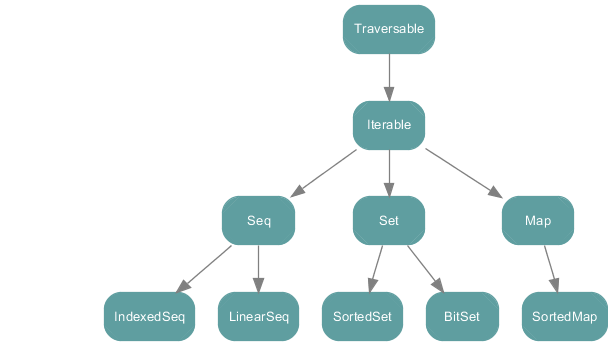
\includegraphics{figures/colls.png}
\caption[All \sv{scala.collection} collections]{Basic collections in \sv{scala.collection}
}
\label{colls}
\end{figure}


This work focuses mainly on \texttt{Seq}'s subtree, since it's where we can get the
most prominent speedups by exploiting the sequences' properties. A sequence is a
kind of iterable that has a length method and whose elements have fixed index
positions, starting from 0.


\section{Scala Compile-Time Reflection Overview}

Scala version 2.10, released in January 2013, introduced a new reflection
subsystem adding both run time and compile metaprogramming capabilities. The new
run-time reflection is much more general and feature complete compared to Java's
reflection. Compile-time reflection is quite rare in mainstream statically typed
programming languages and, currently, it can only be found in more exotic
 languages like Haskell~\cite{sheard_template_2002} and Nemerle~\cite{nemerle:macros}.
 Compile-time reflection enabled the introduction of an experimental version of type-safe
 syntactic macros~\cite{burmako2012scala}. 

Syntactic macro systems work at the level of abstract syntax trees and preserve
the lexical structure of the original program. Macro systems that work at the
level of lexical tokens, like the C preprocessor, cannot preserve the
lexical structure reliably. The most widely used implementations of syntactic
macro systems are found in Lisp-like languages such as Common Lisp, Scheme. 
These languages are especially suited for this style of macro due to their uniform,
parenthesized syntax (known as S-expressions).

Compile-time metaprogramming is a valuable tool for enabling such programming
techniques as:

\begin{itemize}
  \item
    Language virtualization (overloading/overriding semantics of the original
    programming language to enable deep embedding of DSLs)
  \item
    Program reification (providing programs with means to inspect their own code)
  \item
     Self-optimization (self-application of domain-specific optimizations based on
program reification)
  \item
    Algorithmic program construction (generation of code that is tedious to write
    with the abstractions supported by a programming language)
\end{itemize}

This work falls in categories three and four, since we use compile-time
reflection to generate code programmatically for each \texttt{macroMap}/\texttt{macroForeach}
method, specialized at the call-site for optimization reasons.

Scala's compile-time metaprogramming can be used through Scala's new macro
system that allows programmers to write \emph{macro defs}: functions that are
transparently loaded by the compiler and executed during compilation.

Our project is implemented directly in the Scala compiler (scalac), so we can
use most of the available compile-time metaprogramming capabilities directly,
without using macro defs explicitly. In the next chapter we will see how we
achieve it.

Compile-time reflection allows us to create new and/or manipulate
existing abstract-syntax trees (ASTs) \fxfatal{abbr} during the compiler's typechecking phase.
All the new or changed ASTs are re-typechecked, guaranteeing us type-safe
transformations. scalac represents ASTs with objects of type
\sv{scala.reflect.api.Tree} or \sv{scala.reflect.api.Exprs}, which is just a typed-wrapper
of \sv{scala.reflect.api.Tree}. Through the available compiler APIs, we can create,
inspect or change the compiler's \sv{scala.reflect.api.Symbol} and
\sv{scala.reflect.api.Type} objects that are related with these ASTs.

For example, we can create the AST of the Scala expression \sv{x < 10} manually,
either with a macro or directly within scalac, with this code
\sv{Apply(Select(Ident(newTermName("x")), newTermName("\$less"),
List(Literal(Constant(10)))))}. \texttt{Apply}, \texttt{Select}, \texttt{Ident}, \texttt{Literal},
\texttt{Constant} are AST objects themselves of \sv{scala.reflect.api.Tree} type.

Obviously, the AST construction is cumbersome and error-prone. But most probably
it is also wrong. If the AST was generated within an internal scalac method or
within a macro, the returned AST will be inlined and type-checked at the
method/macro call site. But this means that the identifier \texttt{x} will be
type-checked at a point where it is most likely not visible, or in the worst
case they might refer to something else. In the macro literature, this
insensitivity to bindings is called non-hygienic\cite{kohlbecker1986hygienic,nemerle:macros}. Scala's
compile-time reflection solves the non-hygiene problem providing a built-in
macro, called \texttt{reify}, that produces its tree one stage later.

The \texttt{reify} macro plays a crucial role in the compile-time metaprogramming. Its
definition as a member of \texttt{Context} is:

\begin{scalaCode}
def reify[T](expr : T): Expr[T] = macro . . .
\end{scalaCode}

Reify accepts a single parameter expr, which can be any well-typed Scala
expression, and creates a tree that, when compiled and evaluated, will recreate
the original tree expr. So \texttt{reify} is like time-travel: trees get re-constituted
at a later stage. If \texttt{reify} is called from normal compiled code, its effect is
that the AST passed to it will be recreated at run time.
Consequently, if \texttt{reify} is called from a macro implementation or a method inside
scalac, its effect is that the AST passed to it will be recreated at
macro-expansion time (which corresponds to run time for macros). This gives a
convenient way to create syntax trees from Scala code: pass the Scala code to
\texttt{reify}, and the result will be a syntax tree that represents that very same code.

For example, \sv{reify(x < 10)} will generate an \texttt{Expr} object representing the
same AST we created manually before.

More importantly, \texttt{reify} packages the result expression tree with the types and
values of all free references that occur in it. This means in effect that all
free references in the result are already resolved, so that re-typechecking the
tree is insensitive to its environment. All identifiers referred to from
an expression passed to \texttt{reify} are bound at the definition site, and not re-bound
at the call site. As a consequence, macros that generate trees only by means
of passing expressions to \texttt{reify} are hygienic.

So, in a sense, Scala macros are self-cleaning. Their basic form is minimal
and unhygienic, but that simple form is expressive enough to formulate a
\texttt{reify} macro, which in turn can be used to make tree construction in macros
concise and hygienic.

Another important compile-time metaprogramming operation is the \emph{splicing},
which could be described as \texttt{reify}'s inverse operation. Using \texttt{Expr}'s splice
method we can inject an existing AST inside a \texttt{reify}'s body.

Reification and splicing operations are crucial to our implementation, as we
will see in the next chapter.